\documentclass{beamer}

\title{Sufficient Statistics for Welfare Analysis: A Bridge Between Structural and Reduced-Form Methods}
\author{Raj Chetty}
\date{\today}

\begin{document}

\frame{\titlepage}

\begin{frame}
\frametitle{Introduction}
\begin{itemize}
\item Structural Approach: Estimate complete model of behaviour by estimating the parameters of that models. These parameters are independent of regime and you can use these parameters to simulate behaviour under alternative policy regimes. 
\item Reduced Form Approach: This approach estimates treatment effects or response to a specific reform. For instance, what elasticity of labor supply in response to taxation? In some simpler models, you can bring the two closer and potentially back out structural parameters from reduced parameters. 

\end{itemize}
\end{frame}

\begin{frame}
\frametitle{Key Concepts}
\begin{itemize}
    \item Sufficient-statistic: You want to make a statement about behaviour in response to a policy? Sometimes just knowing a specific reduced form parameter is enough to completely understand the behaviour and simulate behaviour. Such a reduced parameter is sufficient statistic. 
    \item Sufficient statistic is a function of primitive parameters and different parameters can have different values but it does not matter in so far as they generate same value of this statistics.
\end{itemize}
\end{frame}

\begin{frame}{Illustrataion}
    \begin{figure}[h]
        \centering
        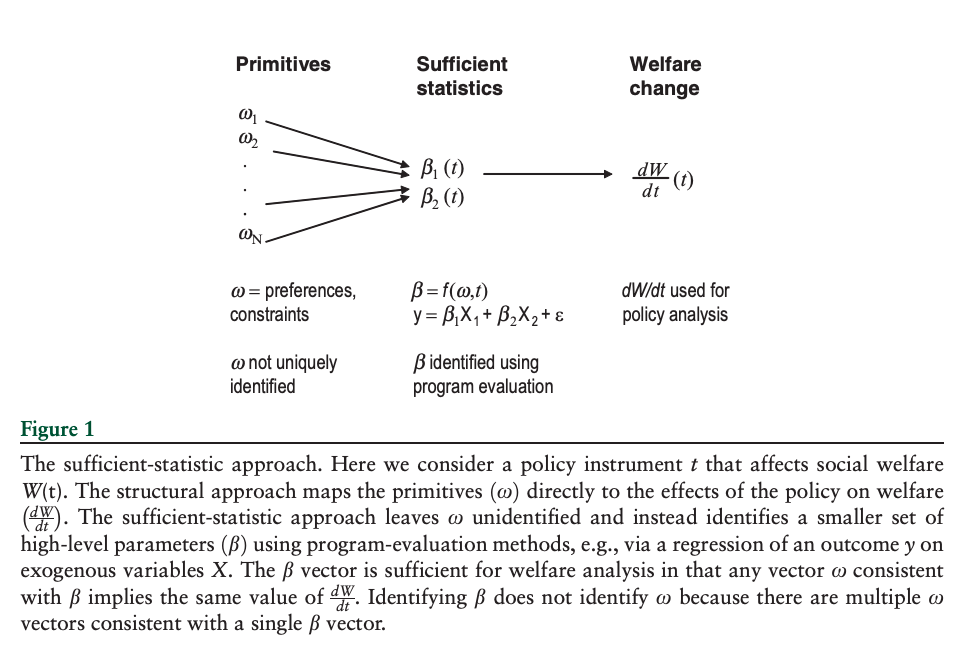
\includegraphics[width =\textwidth]{Paper Presentations/SufficientStatIlustration.png}
        \label{fig:enter-label}
    \end{figure}
\end{frame}

\begin{frame}
\frametitle{Methodology}
\begin{itemize}
    \item Framework of the sufficient-statistic approach.
    \item Key formulas and models.
\end{itemize}
\end{frame}

\begin{frame}
\frametitle{Applications}
\begin{itemize}
    \item Application in income taxation.
    \item Application in social insurance.
\end{itemize}
\end{frame}

\begin{frame}
\frametitle{Behavioral Models}
\begin{itemize}
    \item Application to behavioral economics.
\end{itemize}
\end{frame}

\begin{frame}
\frametitle{Broader Implications}
\begin{itemize}
    \item Potential applications in various economic fields.
\end{itemize}
\end{frame}

\begin{frame}
\frametitle{Conclusion}
\begin{itemize}
    \item Main findings and contributions.
    \item Importance in policy analysis.
\end{itemize}
\end{frame}

\begin{frame}
\frametitle{References}
% Add your references here
\end{frame}

\end{document}
